\section{Model}
\label{sec:model}

\begin{figure}
  \begin{centering}
  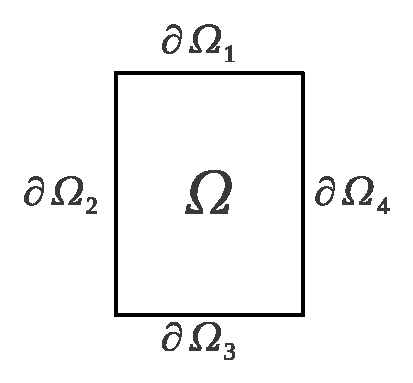
\includegraphics[width=0.2\columnwidth]{domain}
  \caption{\label{fig:domain} Calculation domain $\Omega\subset\mathbb{R}^2$
  	with boundaries $\partial\Omega_{1\ldots 4}\subset\partial\Omega$.}
  \end{centering}
\end{figure}

The model for solving PNP system is implemented in Hermes.
A rectangular 2D domain $\Omega\subset\mathbb{R}^2$ with boundaries 
$\partial\Omega_{1\ldots 4}\subset\partial\Omega$  is considered (see Fig.~\ref{fig:domain}). 
As there is no flow considered into or out from the domain and there is no
constant concentration at the boundaries, zero Neumann boundary conditions were used 
for Eq.~\eqref{eq:nernst-planck}:
\begin{equation}
  -D \frac{\partial C}{\partial n} - z \mu F C \frac{\partial \phi} {\partial n} = 0.
  \label{eq:nernst-planck-boundary}
\end{equation}
As a positive constant voltage $V_{pos}$ was applied on $\Omega_1$ and $V_{neg}=0$ was applied
on $\Omega_3$, Dirichlet boundary conditions were used for Eq.~\eqref{eq:poisson} for
boundaries $\Omega_1$ and $\Omega_3$:
\begin{eqnarray}
  \phi_{\partial\Omega_1}&=&V_{pos},\\
  \phi_{\partial\Omega_3}&=&0,
  \label{eq:dirichlet}
\end{eqnarray}
and Neumann boundaries for $\Omega_2$ and $\Omega_4$:
\begin{equation}
  \frac{\partial \phi_{\Omega_2}}{\partial n}=\frac{\partial \phi_{\Omega_4}}{\partial n}=0.
\end{equation}


\subsection{Weak form of Poisson-Nernst-Planck system}

The initial more implicit version of the derived weak form of PNP
was derived in~\cite{pugal2010spie}.
To make the derivation of the weak forms more convenient, the following
constants are used: 
\begin{eqnarray}
  K & = &z \mu F,\\
  L&=&\frac{F}{\varepsilon}.
  \label{eq:KL}
\end{eqnarray}
So Eq.~\eqref{eq:nernst-planck} and Eq.~\eqref{eq:poisson} become after 
substituting Eq.~\eqref{eq:rho} and the constants $K$ and $L$:
\begin{eqnarray}
  \frac{\partial C}{\partial t}-D\nabla^2 C-K\nabla\cdot \left(C\nabla\phi\right)&=&0,\label{eq:nernst-planck-2}\\
  -\nabla^2\phi-L\left(C-C_{0}\right)&=&0.\label{eq:poisson-2}
\end{eqnarray}
The boundary condition Eq.~\eqref{eq:nernst-planck-boundary} becomes:
\begin{equation}
  -D\frac{\partial C}{\partial n}-KC\frac{\partial\phi}{\partial n}=0.
  \label{eq:nernst-planck-boundary-2}
\end{equation}
The space for solution is $V=H^1\left(\Omega\right)$ where 
$H^1\left(\Omega\right)=\left\{v\in L^2\left(\Omega\right);\ \nabla v \in \left[L^2\left(\Omega\right)\right]^2\right\}$.
Let's choose a test function $v^C\in V$.
The weak form the Nernst-Planck equation Eq.~\eqref{eq:nernst-planck-2}
is found by multiplying it with the test function $v^C$ and then integrating over the domain~$\Omega$:
\begin{equation}
  \int_{\Omega}\frac{\partial C}{\partial t}v^C d\mathbf{x}
  -\int_{\Omega}D\nabla^2Cv^C d\mathbf{x}-\int_{\Omega}K\nabla C\cdot
  \nabla\phi v^C d\mathbf{x} - \int_{\Omega}KC\nabla^2\phi v^C d\mathbf{x}=0.
  \label{eq:nernst-planck-weak1}
\end{equation}
After adding the weak form of the boundary term 
(Eq.~\eqref{eq:nernst-planck-boundary-2}) and applying
the Green's first identity to the terms that contain Laplacian $\nabla^2$ we get
\begin{eqnarray}
 && \int_{\Omega}\frac{\partial C}{\partial t}v^C d\mathbf{x}+
  D\int_{\Omega}\nabla C\cdot\nabla v^C d\mathbf{x}-
  K\int_{\Omega}\nabla C \cdot \nabla \phi v^C d\mathbf{x}+
  K\int_{\Omega}\nabla\left(Cv^C\right)\cdot \nabla \phi d\mathbf{x}\\
  &&-D\int_{\partial\Omega}\frac{\partial C}{\partial n}v^C d\mathbf{S}-
  \int_{\partial\Omega}K\frac{\partial\phi}{\partial n}Cv^C d\mathbf{S}=0.
  \label{eq:nernst-planck-weak2}
\end{eqnarray}
After expanding the nonlinear term and given that the boundary terms
do not contribute, the weak form becomes
\begin{equation}
  \int_{\Omega}\frac{\partial C}{\partial t}v^C d\mathbf{x}+
  D\int_{\Omega}\nabla C \cdot \nabla v^C d\mathbf{x}-
  K\int_{\Omega}\nabla C \cdot \nabla \phi v^C d\mathbf{x}+
  K\int_{\Omega}\nabla \phi \cdot \nabla C v^C d\mathbf{x}+
  K\int_{\Omega} C \left(\nabla\phi\cdot\nabla v^C\right) d\mathbf{x}=0.
  \label{eq:nernst-planck-weak3}
\end{equation}
As the second and third term cancel out, the final weak from of 
the Nernst-Planck equation is
\begin{equation}
  \int_{\Omega}\frac{\partial C}{\partial t}v^C d\mathbf{x}+
  D\int_{\Omega}\nabla C \cdot \nabla v^C d\mathbf{x}+
  K\int_{\Omega} C \left(\nabla\phi\cdot\nabla v^C\right) d\mathbf{x}=0.
  \label{eq:nernst-planck-weak-final}
\end{equation}
Similarly the weak form of Poisson equation Eq.~\ref{eq:poisson-2}
with a test function $v^\phi\subset V$ is:
\begin{equation}
  -\int_{\Omega}\nabla^2\phi v^\phi d\mathbf{x}-\int_{\Omega}LCv^\phi d\mathbf{x}+
  \int_{\Omega}LC_{0}v^\phi d\mathbf{x}=0.
  \label{eq:poisson-weak1}
\end{equation}
After expanding the $\nabla^2$ terms, the final form becomes
\begin{equation}
  \int_{\Omega}\nabla\phi\cdot\nabla v^\phi d\mathbf{x}-\int_{\Omega}LCv^\phi d\mathbf{x}+
  \int_{\Omega}LC_{0}v^\phi d\mathbf{x}=0.
  \label{eq:poisson-weak-final}
\end{equation}


\subsection{Implementation in Hermes}
To implement the system of equations Eq.~\eqref{eq:nernst-planck-weak-final}
and Eq.~\eqref{eq:poisson-weak-final}, the residuals and the Jacobian
matrix were derived. For that, Crank-Nicolson time stepping was
used
\begin{equation}
  \frac{\partial C}{\partial t} \approx \frac{C^{n+1} - C^n}{\tau},
  \label{eq:cranic}
\end{equation}
where $\tau$ is a time step. For the variables $C^{n+1}$ and $\phi^{n+1}$ the
following notation will be used:
\begin{eqnarray}
  C^{n+1} &=& \sum_{k=1}^{N^C} y_k^{C} v_k^{C}, \label{eq:cnotation}j\\
  \phi^{n+1} &=& \sum_{k=1}^{N^{\phi}} y_k^{\phi} v_k^{\phi}\label{eq:phinotation},
\end{eqnarray}
where $v_k^C$ and $v_k^\phi$ are piecewise polynomial functions in $V$.
Considering the Crank-Nicolson time stepping and the notation~\eqref{eq:cnotation},
the time discretized Eq.~\eqref{eq:nernst-planck-weak-final} becomes
\begin{eqnarray}
  F_i^C\left(Y\right) & = & \int_{\Omega} \frac{C^{n+1}}{\tau}v_i^C d\mathbf{x} - 
  \int_{\Omega} \frac{C^{n}}{\tau}v_i^C d\mathbf{x}\nonumber\\
  &&+\frac 12 \left[D\int_{\Omega} \nabla C^{n+1} \cdot \nabla v_i^C d\mathbf{x}+ 
  	D\int_{\Omega} \nabla C^{n} \cdot \nabla v_i^C d\mathbf{x}\right]\nonumber\\
  &&+ \frac 12 \left[K\int_{\Omega}C^{n+1} \left(\nabla \phi^{n+1} \cdot \nabla v_i^C\right) d\mathbf{x}+
  K\int_{\Omega}C^{n} \left(\nabla \phi^{n} \cdot \nabla v_i^C\right) d\mathbf{x}\right]\label{eq:Fc},
\end{eqnarray}
and in the notation~\eqref{eq:phinotation}, Eq.~\eqref{eq:poisson-weak-final} becomes
\begin{equation}
  F_i^{\phi}\left(Y\right) = \int_{\Omega} \nabla \phi^{n+1} \cdot \nabla v_i^{\phi} d\mathbf{x} 
  - \int_{\Omega} LC^{n+1}v_i^{\phi} d\mathbf{x} + \int_{\Omega} LC_0 v_i^{\phi} d\mathbf{x}.
  \label{eq:Fphi}
\end{equation}
For the implementation the $2\times 2$ Jacobian matrix $DF/DY$ with elements corresponding to
\begin{equation}
  \frac{\partial F_i^C}{\partial y_j^C}, \ \frac{\partial F_i^C}{\partial y_j^{\phi}},\  
  \frac{\partial F_i^{\phi}}{\partial y_j^C}, \ \frac{\partial F_i^{\phi}}{\partial y_j^{\phi}},
\end{equation}
must be derived: 
\begin{eqnarray}
  \frac{\partial F_i^C}{\partial y_j^C} &=& 
  \int_{\Omega} \frac{1}{\tau} v_j^C v_i^C d\mathbf{x} + 
  \frac 12 D\int_{\Omega} \nabla v_j^C \cdot \nabla v_i^C d\mathbf{x}
  + \frac 12 K\int_{\Omega} v_j^C \left(\nabla \phi^{n+1} \cdot \nabla v_i^C\right) d\mathbf{x},\label{eq:dFcdyc}\\
  \frac{\partial F_i^C}{\partial y_j^{\phi}} &=&
  \frac 12 K \int_{\Omega} C^{n+1} \left(\nabla v_j^{\phi} \cdot \nabla v_i^C\right) d\mathbf{x},\\
  \frac{\partial F_i^{\phi}}{\partial y_j^C} &=&
  - \int_{\Omega} L v_j^C v_i^{\phi} d\mathbf{x},\\
  \frac{\partial F_i^{\phi}}{\partial y_j^{\phi}} &=&
  \int_{\Omega} \nabla v_j^{\phi} \cdot \nabla v_i^{\phi} d\mathbf{x}\label{eq:dFphidyphi}.
\end{eqnarray}
In Hermes Eq.~\eqref{eq:Fc} and \eqref{eq:Fphi} define the residuum $F$ and
Eq.~\eqref{eq:dFcdyc}---\eqref{eq:dFphidyphi} define the Jacobian matrix $J$.

\subsection{Adaptive multi-mesh solution in Hermes}

The defined Jacobian $J$ and residuum $F$ can be simply solved with Hermes by
using Newton's iteration. However, we were more interested in the automatic
adaptivity to control the error and problem size.

In a traditional low-order FEM, refining an element is not algorithmically complicated,
and so the most difficult part is to find out what elements should be refined. 
To do this, various techniques ranging from rigorous guaranteed a-posteriori 
error estimates to heuristic criteria such as residual error indicators, 
error indicators based on steep gradients, etc are employed. 
Unfortunately, none of these approaches are suitable for real-life 
multiphysics coupled problems or higher-order finite element methods: 
rigorous guaranteed error estimates only exist for very simple problems 
(such as linear elliptic PDE), and moreover only for low-order finite elements 
(such as piecewise linear approximations). These heuristic techniques 
are not employed in Hermes since they may fail 
in non-standard situations, and because they lack a 
transparent relation to the true approximation error.
In order to obtain fast, usable adaptivity, one has to resort to adaptive \emph{hp}-FEM.
Automatic adaptivity in the \emph{hp}-FEM is substantially different from adaptivity 
in low-order FEM, since every element can be refined in many different ways. 
Fig.~\ref{fig:refinements} shows several illustrative refinement candidates for a fourth-order element.
\begin{figure}
  \begin{centering}
  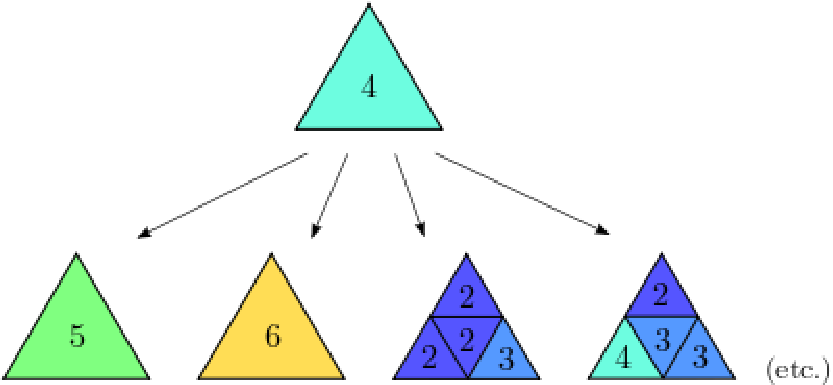
\includegraphics[width=0.5\columnwidth]{refinements}
  \caption{\label{fig:refinements} Refinement candidates for a fourth-order
  element.}
  \end{centering}
\end{figure}
The number of possible element refinements is implementation dependent. 
In general it is very low in \emph{h} or \emph{p} adaptivity, 
but much higher in \emph{hp}-adaptivity, and it rises even more when 
anisotropic refinements are enabled.
Hermes supports 8 different refinement modes, namely,
3 isotropic and 5 anisotropic refinements. The isotropic refinements are
\emph{h}-isotropic (H\_ISO), \emph{p}-isotropic (P\_ISO), \emph{hp}-isotropic (HP\_ISO).
Anisotropic refinement modes are
\emph{h}-anisotropic (H\_ANISO),
\emph{hp}-anisotropic-\emph{h} (HP\_ANISO\_H), \emph{p}-anisotropic (P\_ANISO),
\emph{hp}-anisotropic-p (HP\_ANISO\_P), and \emph{hp}-anisotropic (HP\_ANISO).
Due to the large number of refinement options, classical error estimators 
that provide a constant error estimate per element, cannot be used to 
guide automatic \emph{hp}-adaptivity. 
For this, one needs to know the shape of the approximation error.
Hermes uses a pair of approximations with different orders of accuracy 
to obtain this information: coarse mesh solution and fine mesh solution. 
The initial coarse mesh is read from the mesh file, and the initial 
fine mesh is created through its global refinement both in \emph{h}
and \emph{p}. The fine mesh solution is the approximation of 
interest both during the adaptive process and at the end of computation. 
The coarse mesh solution represents its low-order part.
Here global orthogonal projection of the fine mesh solution 
on the coarse mesh was used instead instead of solving on the coarse mesh.

\begin{figure}
  \begin{centering}
  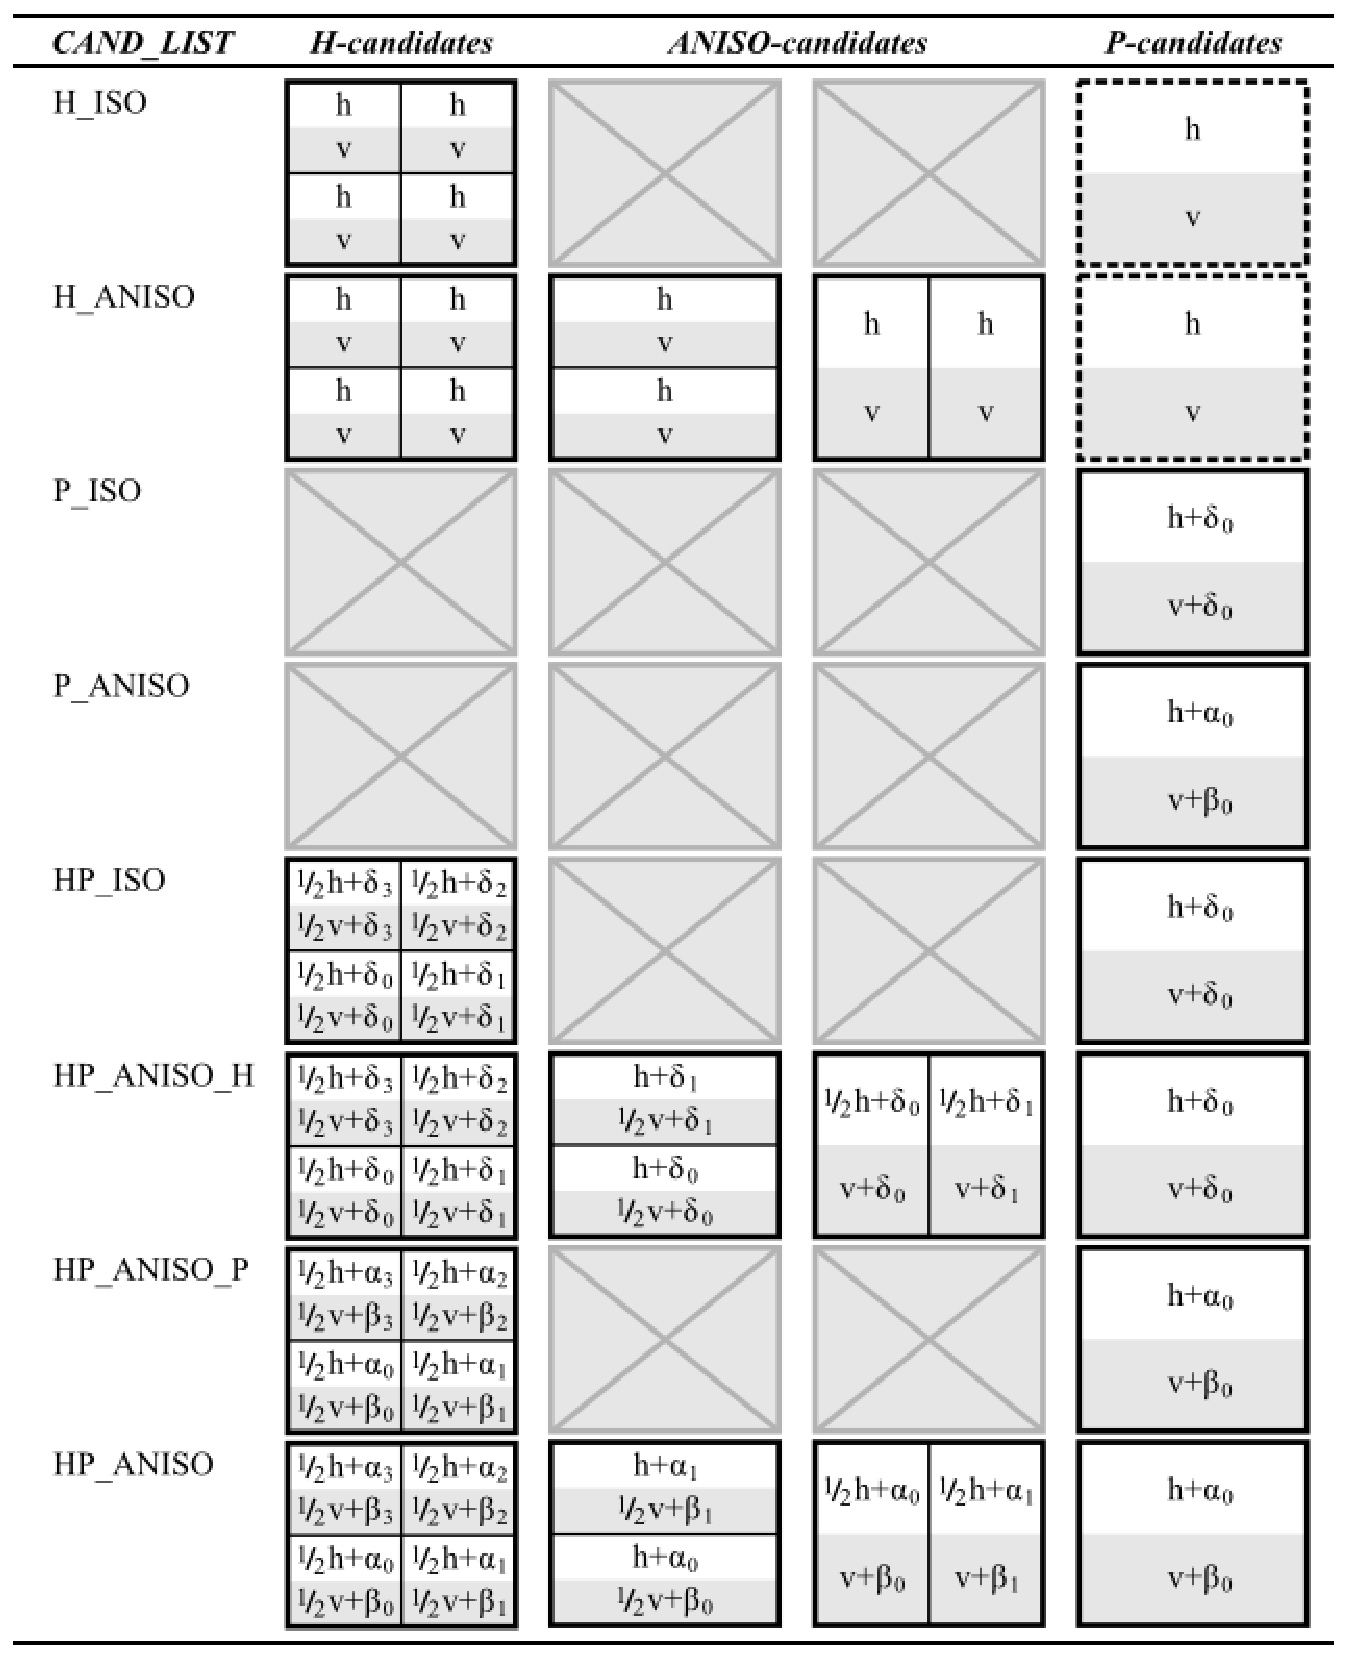
\includegraphics[width=0.5\columnwidth]{cand_list_quads}
  \caption{\label{fig:candlist} Refinement candidates for every
  refinement mode for quad type elements.}
  \end{centering}
\end{figure}
Refinement mode is selected by a user from among 8 modes listed before.
Hermes selects a particular
refinement scheme from several candidates based on the score which is
calculated as follows
\begin{equation}
	s=\frac{\log_{10} e_0 - \log_{10} e}{\left( d_0-d \right)^{\xi}},
\end{equation}
where $e$ and $d$ are an estimated error and an estimated
number of DOF of a candidate respectively, $e_0$ and $d_0$
are are an estimated error and an estimated number of DOF
of the examined element, respectively, and $\xi$ is a
convergence exponent. Here candidate
refers to a proposed refinement. Fig.~\ref{fig:candlist} shows all the proposed
refinements for all refinement modes in case of quad elements.
More information about the refinement modes and technical details
about the score calculation can be found in~\cite{Hermes-project}.

\begin{figure}
  \begin{centering}
  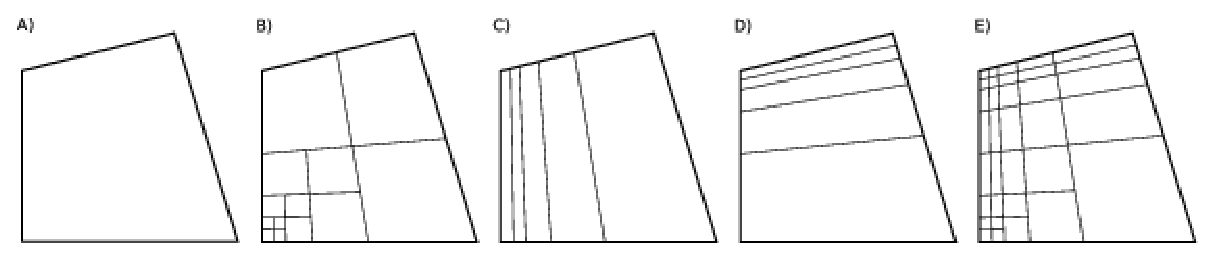
\includegraphics[width=0.5\columnwidth]{multimesh1}
  \caption{\label{fig:multimesh1} Master mesh (A) and 
  three different meshes for a coupled problem (B)~---~(D),
  and the virtual union mesh (E).}
  \end{centering}
\end{figure}
\begin{figure}
  \begin{centering}
  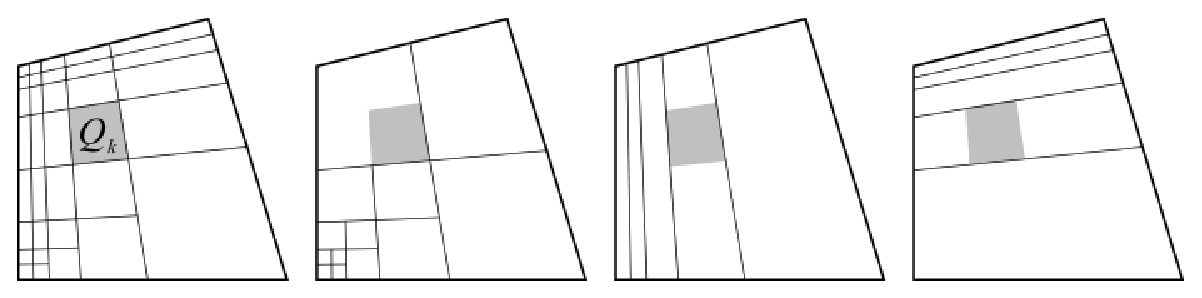
\includegraphics[width=0.5\columnwidth]{multimesh2}
  \caption{\label{fig:multimesh2} Integration over an element
  $Q_k$ of the virtual union mesh and the appropriate subelements
  of the existing elements where this integration is performed.}
  \end{centering}
\end{figure}
In multiphysics PDE systems such as Poisson-Nernst-Planck system it can 
happen that one physical field is very smooth whereas other one is not.
This is well shown in Fig.~\ref{fig:comsol-conc-volt}. 
If all the fields are approximated on the same mesh, then the necessity 
to refine the mesh at the steep gradient of a field implies new degrees 
of freedom for the smooth fields as well. This can be very wasteful.
Hermes makes it possible to approximate them on individual meshes. 
These meshes are not completely independent of each other --- they have 
a common coarse mesh that we call master mesh. The master mesh is 
there for algorithmic purposes only, it may not even be used for 
discretization purposes: Every mesh in the system is obtained from 
it via an arbitrary sequence of elementary refinements. 
This is illustrated in Fig.~\ref{fig:multimesh1}, where (A) is the master mesh, 
(B)~---~(D) three different meshes (say, for a coupled problem with three equations),
and (E) is the virtual union mesh that is used for assembling.
The union mesh is not constructed physically in the computer 
memory --- it merely serves as a hint to correctly transform  the 
integration points while integrating over sub-elements of an elements 
of the existing meshes. Fig.~\ref{fig:multimesh2} shows the integration
over an element $Q_k$ of the virtual union mesh.
As a result, the multimesh discretization of the PDE system is 
monolithic in the sense that no physics is lost --- all integrals 
in the discrete weak formulations are evaluated exactly up to 
the error in the numerical quadrature. 

